
For the following instructions to work you need to have your Prophet 600 connected via MIDI to a device where you can manage MIDI SysEx files, e.g. receive, store and send. Make sure that the MIDI receive channel on the Prophet 600 and the MIDI send channel of the sending device are the same (see section \ref{midiintegration}).

In \presetmode the Prophet 600 loads patch data is receives via MIDI into the active controls. This is like loading a patch from memory where the panel controls may not (and typically don't) show the values of the patch being played. You can edit and store the patch in the normal way. This way of loading a patch is useful if you want to try out a patch from MIDI SysEx before deciding if it should be kept and without having to allocate a storage number in memory. The prophet 600 will never write incoming patch MIDI SysEx to memory unless the \patchmgmt is activated. 

\textbf{Patch Management Mode}

In order to manage patches in memory via SysEx you need to enter the \patchmgmt. In this mode any patch data received via MIDI SysEx is loaded directly into the storage number as indicated in the SysEx data. This extends to the load of the entire patch bank. In patch management mode you can also dump single patches as well as the entire patch bank. 

To enter the patch management mode use \shiftmode or \shiftlock and press the \record button. The \patchmgmt is indicated by a flashing \preset button. To leave the mode, press the \record button. 

\scalebox{0.4}{
  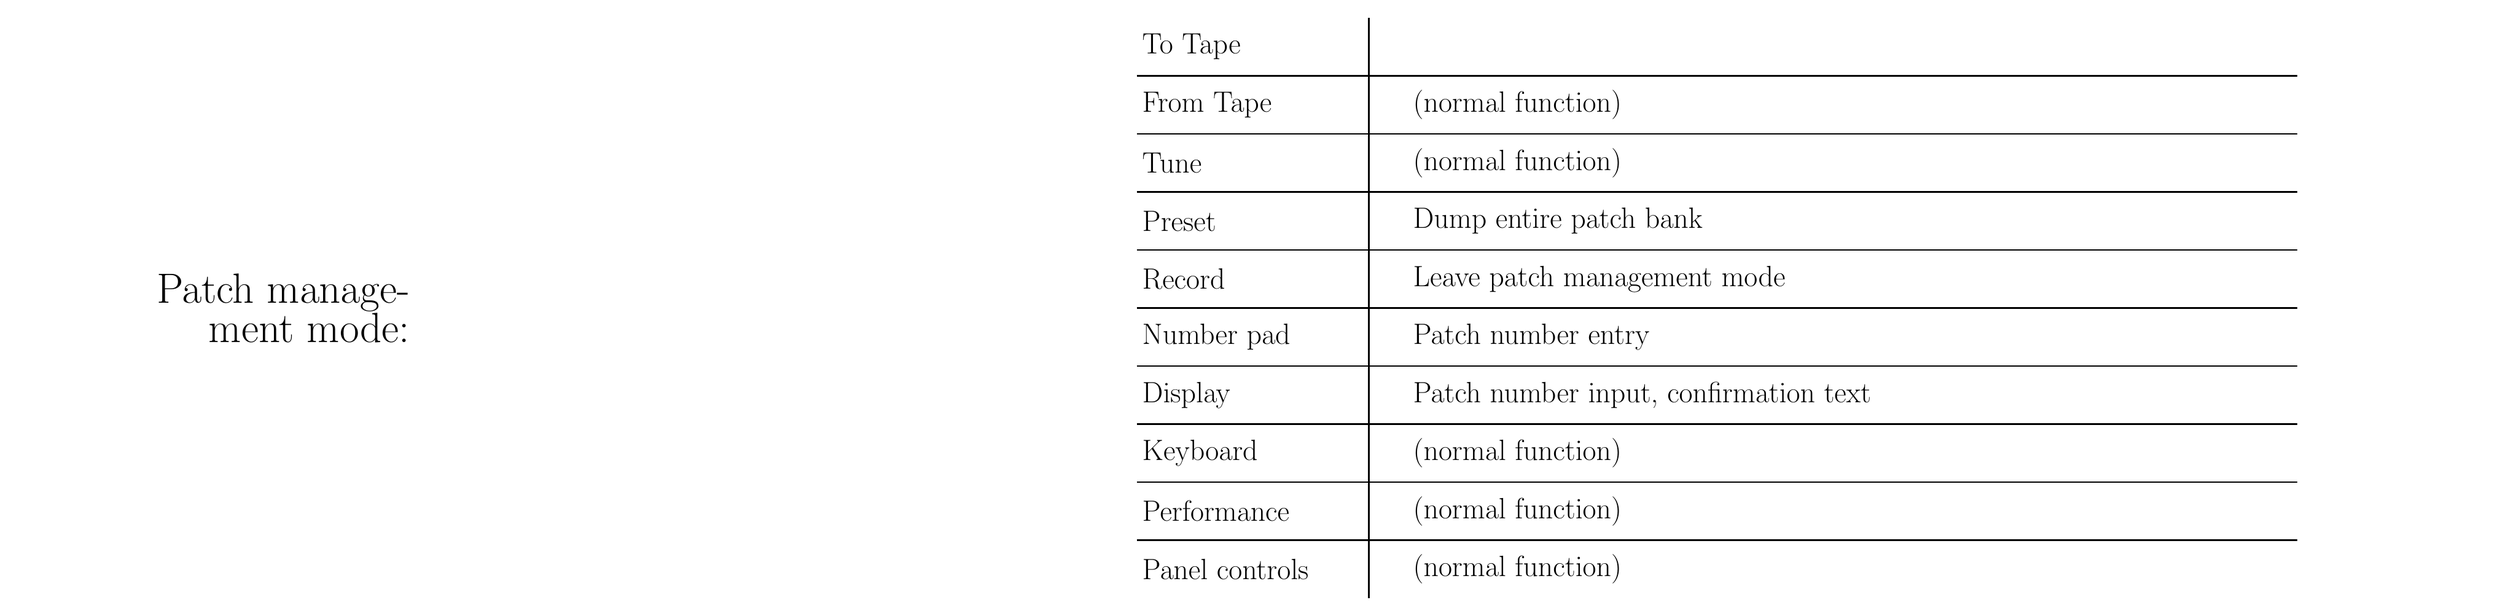
\begin{tikzpicture}[scale=0.8]
  \node[font=\fontsize{26}{22}\selectfont, align=right, outer sep=0.5mm, anchor = west, text width=8cm] at (0cm,12cm) {Patch management mode:};
    \upperbuttons{13cm,7cm}{P}{P}

    \node[font=\fontsize{18}{22}\selectfont, align=left, outer sep=0.0mm, anchor = west, text width=8cm] at (29cm,5.25cm) {Panel controls};
    \node[font=\fontsize{18}{22}\selectfont, align=left, outer sep=0.0mm, anchor = west, text width=22cm] at (36cm,5.25cm) {(normal function)};
    \draw[line width=1pt]++(29cm,6cm)--++(30cm,0cm);     
    \node[font=\fontsize{18}{22}\selectfont, align=left, outer sep=0.0mm, anchor = west, text width=8cm] at (29cm,6.75cm) {Performance};
    \node[font=\fontsize{18}{22}\selectfont, align=left, outer sep=0.0mm, anchor = west, text width=22cm] at (36cm,6.75cm) {(normal function)};
    \draw[line width=1pt]++(29cm,7.5cm)--++(30cm,0cm);     
    \node[font=\fontsize{18}{22}\selectfont, align=left, outer sep=0.0mm, anchor = west, text width=8cm] at (29cm,8.25cm) {Keyboard};
    \node[font=\fontsize{18}{22}\selectfont, align=left, outer sep=0.0mm, anchor = west, text width=22cm] at (36cm,8.25cm) {(normal function)};
    \draw[line width=1pt]++(29cm,9cm)--++(30cm,0cm);     
    \node[font=\fontsize{18}{22}\selectfont, align=left, outer sep=0.0mm, anchor = west, text width=8cm] at (29cm,9.75cm) {Display};
    \node[font=\fontsize{18}{22}\selectfont, align=left, outer sep=0.0mm, anchor = west, text width=22cm] at (36cm,9.75cm) {Patch number input, confirmation text};
    \draw[line width=1pt]++(29cm,10.5cm)--++(30cm,0cm);     
    \node[font=\fontsize{18}{22}\selectfont, align=left, outer sep=0.0mm, anchor = west, text width=8cm] at (29cm,11.25cm) {Number pad};
    \node[font=\fontsize{18}{22}\selectfont, align=left, outer sep=0.0mm, anchor = west, text width=22cm] at (36cm,11.25cm) {Patch number entry};
    \draw[line width=1pt]++(29cm,12cm)--++(30cm,0cm);     
    \node[font=\fontsize{18}{22}\selectfont, align=left, outer sep=0.0mm, anchor = west, text width=8cm] at (29cm,12.75cm) {Record};
    \node[font=\fontsize{18}{22}\selectfont, align=left, outer sep=0.0mm, anchor = west, text width=22cm] at (36cm,12.75cm) {Leave patch management mode};
    \draw[line width=1pt]++(29cm,13.5cm)--++(30cm,0cm);  
    \node[font=\fontsize{18}{22}\selectfont, align=left, outer sep=0.0mm, anchor = west, text width=8cm] at (29cm,14.25cm) {Preset};
    \node[font=\fontsize{18}{22}\selectfont, align=left, outer sep=0.0mm, anchor = west, text width=22cm] at (36cm,14.25cm) {Dump entire patch bank};
    \draw[line width=1pt]++(29cm,15cm)--++(30cm,0cm);  
    \node[font=\fontsize{18}{22}\selectfont, align=left, outer sep=0.0mm, anchor = west, text width=8cm] at (29cm,15.75cm) {Tune};
    \node[font=\fontsize{18}{22}\selectfont, align=left, outer sep=0.0mm, anchor = west, text width=22cm] at (36cm,15.75cm) {(normal function)};
    \draw[line width=1pt]++(29cm,16.5cm)--++(30cm,0cm);  
    \node[font=\fontsize{18}{22}\selectfont, align=left, outer sep=0.0mm, anchor = west, text width=8cm] at (29cm,17.25cm) {From Tape};
    \node[font=\fontsize{18}{22}\selectfont, align=left, outer sep=0.0mm, anchor = west, text width=22cm] at (36cm,17.25cm) {(normal function)};
    \draw[line width=1pt]++(29cm,18cm)--++(30cm,0cm);  
    \node[font=\fontsize{18}{22}\selectfont, align=left, outer sep=0.0mm, anchor = west, text width=8cm] at (29cm,18.75cm) {To Tape};
    \node[font=\fontsize{18}{22}\selectfont, align=left, outer sep=0.0mm, anchor = west, text width=22cm] at (36cm,18.75cm) {};
    
    \draw[line width=1pt]++(35cm,4.5cm)--++(0cm,15cm);  

  \end{tikzpicture}
}


\textbf{Dumping the patch library as SysEx} 

To dump the entire patch bank press the \preset button. The screen will scroll a confirmation message. Note, however, that only valid presets are exported. Any unused patch slots are skipped.

\textbf{Dumping single patches as SysEx} 

To dump a single patch in patch management mode simply enter the patch number on the number pad. Note, that if there is no valid patch data stored in the selected patch slot, the entry will be accepted but there will be no dump.

Note: the Prophet 600 also supports MIDI dump requests. When sending a SysEx patch request for a particular patch number to the Prophet 600 you will receive the corresponding single SysEx back (on the specified MIDI send channel) provided the specified patch number is between 0 and 99 and a valid patch is stored at this number. This can be done in all modes at any time, not just in \patchmgmt.

\textbf{Loading patches} 

Loading MIDI SysEx patches to storage is done by sending the patch SysEx containing the data to the Prophet 600 in \patchmgmt. Each patch contains a patch number. If the patch number is  between 0 and 99 the data will stored in that patch slot overwriting the existing stored patch. Therefore, loading a SysEx patch library will overwrite the entire library stored on the Prophet 600 when \patchmgmt is activated. When a patch has been loaded to storage the number of the patch number is shown on the display.

In normal \presetmode patch MIDI is only loaded into the active control values as described above. In \livemode incoming patch MIDI SysEx is ignored. Requiring \patchmgmt to be activated for MIDI-to-storage operations protects your patches from accidental overwrite. Still, it is always advisable to regularly archive patches in SysEx files outside the instrument.
